\documentclass{article}
\usepackage[margin=0.75in]{geometry}
\usepackage{graphicx}
\usepackage{calc}  % For width and height calculations
\usepackage{enumitem}
\title{BuckAI Observatory Proposal}
\author{Joachim Moortgat}
\date{\today}
\usepackage{titling}
\pagestyle{empty}


\begin{document}

\noindent
\begin{minipage}{0.8\textwidth}
  \vspace{0pt}
  \begin{center} {\LARGE \bfseries BuckAI Observatory --- White Paper}\\[0.5em]
  {\large Joachim Moortgat}\\
  {\normalsize \today}
  \end{center}
\end{minipage}%
%\hfill
\begin{minipage}[t]{0.2\textwidth}
  \vspace{-6em}
  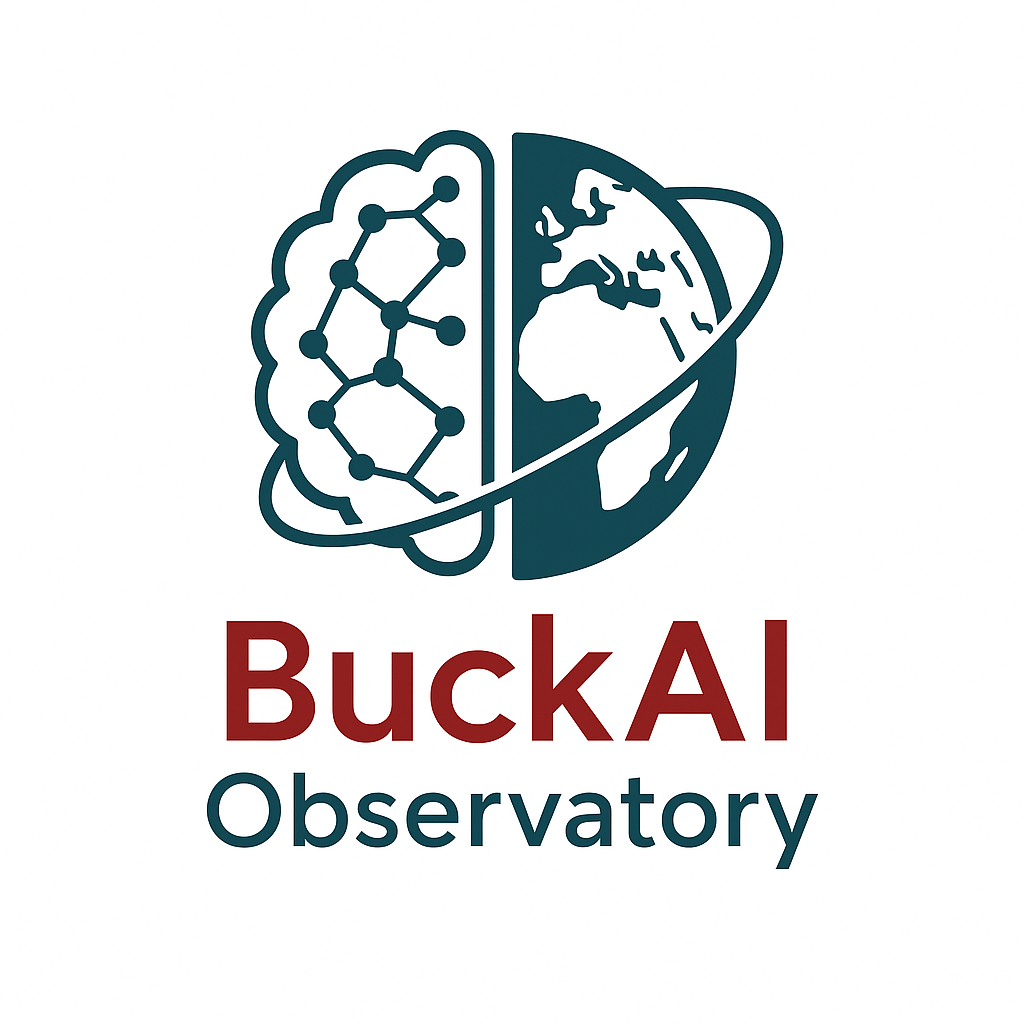
\includegraphics[width=\linewidth]{BuckAI_logo}
\end{minipage}

\noindent
The Ohio State University is positioning itself as a national leader in artificial intelligence (AI) research and education. Multiple successful centers already advance fundamental AI methods and the supporting cyberinfrastructure---for example, TDAI, ICICLE, AI‐EDGE, CQISE, CDME, and Imageomics. To complement these strengths I propose an \emph{applied} AI center, tentatively named the \textbf{BuckAI Observatory}, housed in the College of Arts and Sciences (ASC). This center will focus on Earth Observation AI applications to further research in Earth and Environmental Science and Geodesy and attracting more students into the Earth Sciences and Geodesy programs. 

\section*{Objectives}
\begin{enumerate}[label=\arabic*.]
%\item \textbf{Catalyze interdisciplinary collaboration.}\\
%Bring together OSU researchers who rely on remote sensing with AI method experts in, e.g., Computer Science and Engineering. By fostering relationships \emph{before} external funding calls emerge, we can respond rapidly to short‐lead opportunities. This collaboration is deliberately symbiotic: remote‐sensing science benefits from state‐of‐the‐art AI algorithms, while the rich, multi‐modal and temporally stacked satellite record provides Computer Vision scholars with novel, challenging data far beyond standard RGB imagery and video.
\item \textbf{Catalyze interdisciplinary collaboration.}\\
Bring together OSU researchers who rely on remote sensing with AI method experts in, e.g., Computer Science and Engineering. Special emphasis will be placed on building bridges across the College of Arts and Sciences, the College of Food, Agricultural, and Environmental Sciences (CFAES), and other campus units. By fostering relationships \emph{before} external funding calls emerge, we can respond rapidly to short‐lead opportunities. This collaboration is deliberately symbiotic: remote‐sensing science benefits from state‐of‐the‐art AI algorithms, while the rich, multi‐modal and temporally stacked satellite record provides Computer Vision scholars with novel, challenging data far beyond standard RGB imagery and video.

\item \textbf{Lower the barrier to AI‐enabled remote sensing.}    \begin{itemize}[leftmargin=*]
    \item Expand the ASC Unity cluster with $\sim 10 $ high‐end multi‐GPU nodes and up to a petabyte of shared storage so project teams can access common datasets and reproducible code.
    \item Coordinate with the Ohio Supercomputer Center to optimise storage, compute access and technical support.
    \item Employ a shared data engineer to manage acquisition, pre‐processing and fusion of multi‐sensor data, and to establish best practices in version control and documentation.
    \item Offer a  pool of hourly undergraduate support for manual training datasets that seed larger grant proposals.
    \item Provide short courses, boot camps and annual workshops that couple hands‐on training with research dissemination and “red‐team” proposal reviews (in partnership with ERIK).
    \item Coordinate AI‐related curriculum development to better prepare ASC students for an AI‐driven workforce.
    \end{itemize}

\item \textbf{Develop foundation models for Earth Observation.}\\
Leverage the Observatory's compute and data resources to pre‐train self‐supervised neural networks on vast, multi‐modal, time‐stacked satellite archives, enabling efficient transfer learning for diverse science problems.

\item \textbf{Forge durable external partnerships for a diversified funding portfolio.}
\begin{itemize}[leftmargin=*]
\item Engage the Dean’s Advisory Committee and unit‐level advisory boards to establish a Joint Industry Consortium, in which member companies receive early access to cutting‐edge research through annual workshops and reports.
\item Collaborate with the Technology Commercialization Office to educate investigators on intellectual‐property protection and entrepreneurial pathways.
\end{itemize}
\end{enumerate}

\vspace{0.5em}
\noindent
%\textbf{Return on Investment.}\;Strategic seed funding from ASC will catalyze the research programs of over ten affiliated faculty and, conservatively, enable over \$10M in external funding proposals within five years. These gains will be driven by cross-disciplinary, multi-department, and multi-college collaborations in AI-enhanced remote sensing and beyond.

\textbf{Return on Investment.}\;Strategic seed funding from ASC will catalyze the research programs of over ten affiliated faculty and, conservatively, enable over \$10M in external funding proposals within five years. These gains will be driven by cross-disciplinary, multi-department, and multi-college collaborations in AI-enhanced remote sensing and related fields. Beyond research, the Observatory will enrich student training, modernize curriculum development, and foster industry partnerships through joint consortia and technology transfer—positioning OSU as a national leader in applied AI for Earth and environmental science.


\end{document}




\documentclass{article}
\title{BuckAI Observatory Proposal}
\author{Joachim Moortgat}
\date{\today}

\usepackage{graphicx}


\begin{document}
\maketitle
\centerline{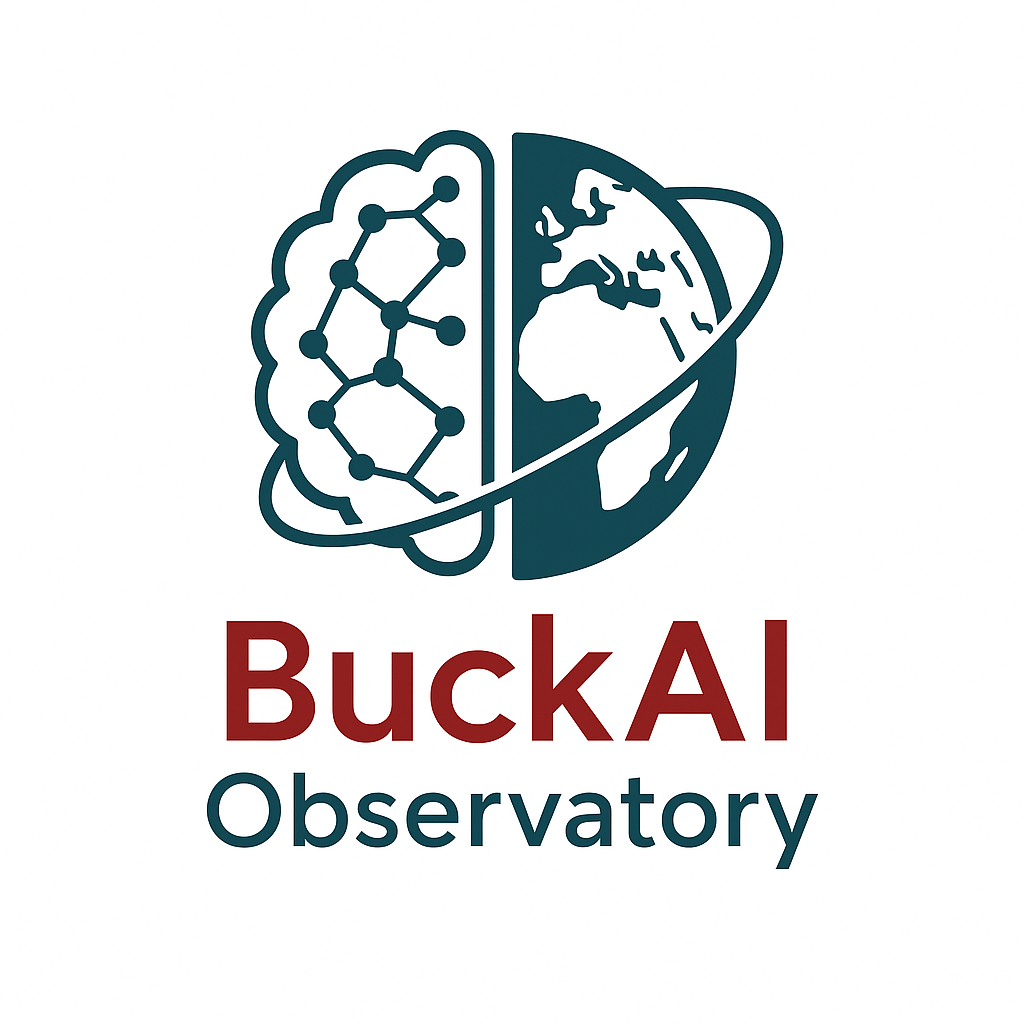
\includegraphics[width=0.3\textwidth]{BuckAI_logo}}

The Ohio State University is striving to establish itself as a national leader in AI research and education. Already, OSU houses several successful centers and institutes that advance AI research (e.g., TDAI, ICICLE, AI-EDGE, CQISE, CDME, Imageomics, ACCAD) with a strong focus on developing cutting-edge AI algorithms and cyberinfrastructure. I propose to complement those strengths with an \textit{applied} AI center housed in the College of Arts and Sciences (ASC) with a primary focus on Earth Observation but also welcoming other AI research related to, e.g., the microbiome and the Arts. To achieve this, I am requesting a significant investment by ASC to provide a backbone of infrastructure and personnel that is hard to write into individual federal grant proposals.

The objectives of such a new Center of Excellence (tentatively dubbed BuckAI Observatory) are to
\begin{itemize}
\item Bring together the many OSU researchers that use remote sensing data in their research and foster collaborations between AI experts in, e.g.,  Computer Science and Engineering, with applied research across ASC and the Food, Agriculture and Environmental Science College. The goal is to establish such potential partnerships long before specific external funding calls are announced, often with a short lead-time. This is envisioned as a symbiotic relationship: not only will remote sensing research benefits from experts in AI algorithms, but multi-modal (e.g., optical, microwave, radar, LIDAR, gravity, magnetic fields, etc.), time-stacked repeat geospatial data also offer a new frontier in AI research beyond RGB images and videos that currently drive much of Computer Vision AI research. 
\item Remove barriers to use remote sensing data in general and to adopt AI to accelerate such research in particular by:
\begin{itemize}
\item Providing shared data storage and computational resources within OSU by expanding the ASC HCP cluster, Unity, with 10 powerful multi-GPU nodes and up to 1 petabyte of storage, such that PIs can more easily share the same remote sensing data and algorithms across projects. Currently, the same or similar satellite data is downloaded an pre-processed by many groups and machine/deep learning algorithms developed by students and postdocs is not necessarily easily accessible when such scholars leave for the next stages in their careers. These proposed resources would be managed by the Observatory to be exclusive for AI-powered research.
\item In parallel, partner with the Ohio Supercomputer Center (OSC) for technical support and optimized access to storage and computational resources. 
\item Provide a shared data-engineer to streamline data acquisition, pre-processing, and fusing across satellite modalities, and establish best practices in data management, code version control and documentation. 
\item Provide a shared pool of funding for hourly undergraduate wages to generate manually labeled training data for pilot projects in the pursuit of larger external funding. 
%\item Facilitate collaborations between remote sensing domain experts and scholars with interest and expertise in the latest state-of-the-art in AI algorithms,  to establish such collaborations.
\item Provide training to faculty/students/postdocs interested in adopting AI into their research.
\item Hold annual workshops in which affiliated researchers can disseminate their AI research across campus and receive feedback from likeminded colleagues (combined with the aforementioned training, and boot-camp sessions).
\item Provide opportunities for `red team' proposal reviews in partnership with, e.g., ERIK.
\item Streamline curriculum development related to AI as part of our educational mission to prepare our students for the modern job market.
\end{itemize}
\item Collaboratively work towards `Foundation Models' in which AI algorithms are pre-trained on massive sets of multi-modal  time-stacked satellite data by self-supervised neural networks, before being fine-tuned (transfer learning) for specific science and engineering problems. 
\item Work with the Dean's Advisory Committee and other such committees across campus (such as the School of Earth Sciences' Alumni Advisory Committee) to seek out industry partnerships that can supplement federal grants in the current tumultuous funding landscape. The most effective path would be to form a Joint Industry Consortium of a dozen companies that pay annual memberships for early access to cutting-edge fundamental and applied AI research at OSU, presented in reports and annual workshops, in parallel with funding specific research projects through Sponsored Research Agreements (SRAs).
\item Partner with OSU's Technology and Commercialization Office (TCO) to educate affiliated researchers on entrepreneurship and opportunities offered through Intellectual Property commercialization (e.g., patents and licensing of AI technologies). Together with the previous point, these are pilot efforts in providing a test-bed for a diversified funding portfolio for AI research.
\end{itemize}

Needless to say, ASC expects a meaningful Return on Investment on their foundational investment (proposed as $\sim 1$M\$). I have argued that removing barriers to incorporating AI into remote sensing powered scientific research across at least ten affiliated faculty should help catalyze at least \$10M in external funding over 5 years. 


\end{document}